\section{Domain Informed Oracle} 

We tackle the challenge of finding a systematic method to map a state to a numerical value: a reward. 
To do so, we make use of the fact that rewards are domain dependent and thus, given domain specific rules, a \emph{domain informed} module can guide a RL agent towards better decisions. This can be done by 
adapting the reward function. For instance, we consider defining which states are desirable, which are to be avoided and which are fatal. Given rules and judgments, a logic programming module 
is able to search the space and send feedback to the reinforcement learning agent. The goal is a systematic method to design a reward function which can ensure faster and more efficient 
training. This knowledge can furthermore be incorporated into resolving the exploration vs. exploitation dilemma. For instance, if a domain informed module 
can infer that only one of the possible next states is desirable, then exploration in that specific case is suboptimal.  
We will call the proposed module a \emph{Domain Informed Oracle}
(\dio{}).

\begin{figure}[H]
  \centering
  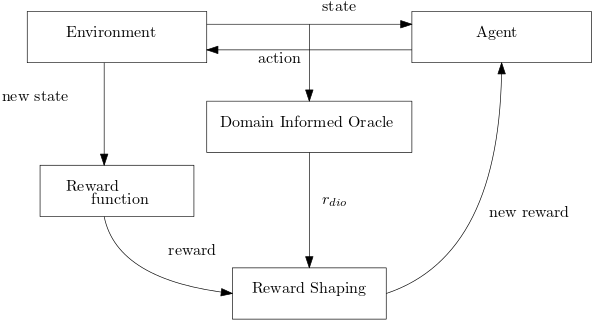
\includegraphics[scale=0.45]{figures/overview.png}
  \caption{Overview of the proposed solution}
  \label{fig:overview}
\end{figure}


The diagram in Figure~\ref{fig:overview} is a high-level description of our proposed solution. 
%
Precisely, the (state, action) pair is fed into \dio{}. While the environment produces its own 
reward function, \dio{} also computes its own reward. 

We could leave the \emph{reward shaping} unit as a design choice. However, it will be enforced in~\ref{sec:comreward}
that whether it is left as a design choice or else, is irrelevant given how \dio{} affects the final results.

\subsection{Architecture}
In this section, we lay the foundations of the architecture that combines the Domain Informed Oracle with 
reinforcement learning. Note that in our proposed architecture, we suppose Proximal Policy Optimization~\cite{schulman17ppo}. 
It does not mean that our solution is specific to it, rather it can be generalized to any algorithm choice.

\begin{figure}[H]
  \centering
  \begin{minipage}{.5\textwidth}
    \centering
    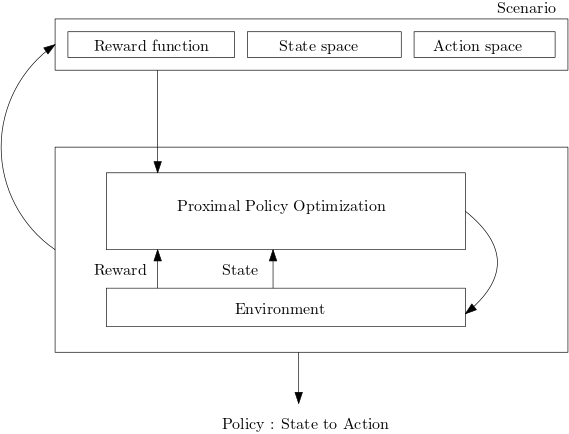
\includegraphics[width=1\linewidth]{figures/basicrl.png}
    \captionof{figure}{Reinforcement learning architecture}
    \label{fig:basicrl}
  \end{minipage}%
  \begin{minipage}{.45\textwidth}
    \centering
    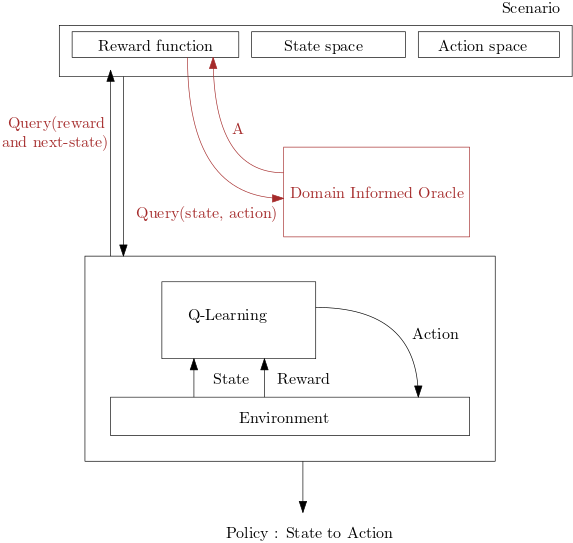
\includegraphics[width=1\linewidth]{figures/dio.png}
    \captionof{figure}{\dio{}+RL architecture}
    \label{fig:diorl}
  \end{minipage}
\end{figure}

The diagram in Figure \ref{fig:basicrl} describes the basic routine of RL in more details. The environment defined by the scenario sends the current state 
to the \emph{Proximal Policy Optimization} algorithm. The agent chooses an action from the action space and sends it to the environment. This action affects the environment stepping it to some next state. 
The resulting state along its associated reward is computed from the reward function and step function formalized in the scenario. Thus, in the next iteration, the 
agent receives the reward from its previous action which it uses to improve its policy and continues with its training starting from the computed next state.  

The architecture in Figure \ref{fig:diorl} introduces \dio{} in the feedback loop. It is kept independent of the RL module. Precisely, when the scenario is query-ed for the reward and 
the resulting next state of a (state, action) pair, rather than computing the reward using the reward function, the latter is able to query \dio{}. The result of this query is $J$: a numerical value 
we defined as $r_\dio{}$, the reward given by \dio{} to the (state, action) pair. More on how this reward is computed in \ref{sec:comreward}.
 

\subsection{\dio{} procedure}
\label{sec:modules}
In practice, we consider the following modules and their interactions as shown in \ref{fig:mods}.


\begin{multicols}{2}
\begin{enumerate}
  \item \textbf{World Rules} defining the rules governing the world. This is domain-dependent and implemented 
        in a logic programming file, i.e. we are able to define the next step via step semantics.
  \item \textbf{Knowledge Base} defining the ground facts which describe the world at a given time step. This module is 
        continuously updated to account for the dynamics of the
        state.
  \item \textbf{Labels} i.e., textual ``norms'' corresponding to an
  iteration of the state. In practice, they are all possible judgments on the resulting state, e.g. \textit{crash :- obs(X,Y), agent(X,Y)}, 
                  or \textit{maybecrash :- nextObs(X,Y), agent(X,Y)}. 
                    Those labels have probabilities associated with
                    them and indicators. Precisely, an indicator over a negative state is $-1$. 
  \item \textbf{Translation Unit} defining the translation from state to ground facts and from labels to a numerical value, e.g. if the predicate crash is true with $P = 0.25$, then the reward shaped is $r + -0.25$. 
  \item \textbf{Reinforcement Learning} is our independent module that does not make assumption on the algorithm chosen for RL.
\end{enumerate}
\end{multicols}


\begin{figure}[H]
  \centering
  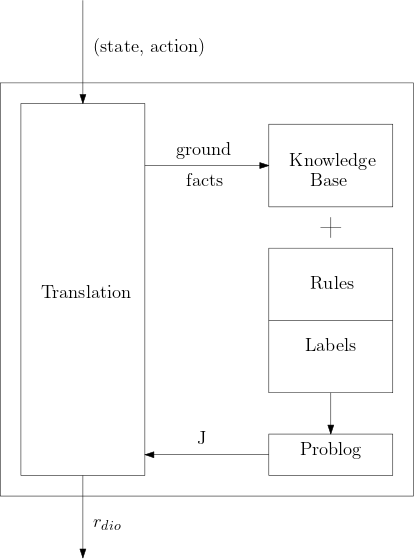
\includegraphics[scale=0.4]{figures/dynamics.png}
  \caption{Modules \& Interactions}
  \label{fig:mods}
\end{figure}

Figure \ref{fig:mods} describes the interactions of the different modules. Precisely, 
given the rules and the world knowledge base at a given time $t$, we are able 
to produce the corresponding label, i.e. the query over a predicate. The predicate is fed 
into the Translation Unit (TU) that transforms the predicate to a numerical value that is given to the Reinforcement Learning 
as a reward shaping $r'$. . Note that the inference on the query is done by a declarative tool that incorporates 
probabilities called \emph{Problog} that we introduce in \ref{sec:problog}.


\subsection{Problog Procedure} 
\label{sec:problog}
% High level overview of Problog
Problog is a logic programming language that aims to bridge between probabilistic 
logic programming and statistical relational learning \cite{fierens_van}. 
A problog program specifies a probability distribution over possible worlds. 
This probability distribution corresponds to the possible worlds whether a fact is taken 
or discarded given the probability associated with it. Precisely, they define a world 
is a subset of ground probabilistic facts where the probability of the subset is the product of 
the probabilities of the facts it contains.

\paragraph{Statistical Relational Learning (SRL)}
    Discipline of Artificial Intelligence that considers first order logic relations between 
    structures of a complex system and model it through probabilistic graphs such as Bayesian or 
    Markov networks.

\paragraph{Probabilistic Logic Programming (PLP)}
    Discipline of Programming Languages that augments traditional logic programming such as Prolog 
    with the power to infer over probabilistic facts to support the modeling of structured 
    probability distributions.


% Evidence and inference tasks in Problog
Furthermore, problog extends PLP with the power of considering evidences 
in the inference task. This is made possible without requiring the transformation 
the Bayesian networks on which to use SRL. Instead, problog considers the subset described above 
and assumes only worlds where the evidence held remains true. Those possible worlds and their associated 
probabilities are then added and divided by the choice with the higher probability. Problog makes this 
possible by a 3-steps conversion from a problog program to a weighted boolean formula.

% Conversion steps to weighted formula
First, problog grounds the program by only considering facts relevant to the query in question. 
The relevant ground rules are specifically converted to equivalent Boolean formulas. 
Precisely, inferences are converted into bi-directional implications and its corresponding premises 
are converted to a conjunction of disjunction of facts. 
Finally, problog asserts the evidence by adding it to the previous boolean formula 
as a conjunction and defines a weight function that assigns a weight to every literal. 
The weights are derived from the probability associated with the relevant literal, whether explicility 
given or implicility computed. 

% How exactly are we getting this numerical value?
\subsection{Computation of Final Reward}
\label{sec:comreward}
In general, reward shaping is expressed as follows
  $R = r_{rl} + r'$, 
such that $r_{rl}$ is the original reward defined by the reinforcement learning environment. Usually, this associates the value of $1$ for a positive terminal state, 
and $-1$ for a negative terminal state. $r'$ is the human bias, i.e. what is added to "shape" the reward function. 
Although only rewarding terminal states is enough to 'reach' a policy that will minimize its losses, it is important to note that a reward function should consider the cost of a 'step' 
for optimal and fast training. The cost of a step is dependent on the state given at that step. For instance, an autonomous vehicle stopping with not cars around, is different from a vehicle 
stopping while a car is behind it. Although the states are not 'terminal', i.e. they do not end an episode, they have different weights. 
An optimal reward function is one that considers those differences. A logic programming module allows us to infer over states using a knowledge base and world rules seamlessly. 

Precisely, let's consider the following example in figure~\ref{fig:diospecs}.
Our agent is running away from a predator. It is currently at position $(0,0)$, and decides to go right, to escape. 
Since, it is a stochastic environment, there is a 0.1 chance that his parts might fail and he stays in the same spot, thus getting eaten by the predator. 
This is easily expressed in a \emph{problog} as follows. 
\begin{verbatim}
  0.9 :: pos(X+1, Y) :- direction(right), pos(X, Y). 
  0.1 :: pos(X, Y) :- direction(right), pos(X, Y). 
\end{verbatim}
Consequently, there is a 0.9 chance that we end up in a 'desirable' state, and a 0.1 chance that we end up in an 'undesirable' state. Precisely, 
\[ 
   r'_{\dio{}} = \sum_{L} Pr[L \mid (s_t, a_t)] I[L]
\] 
Desirable and undesirables are labels noted by 'L'. We identify their indicator $I[L]$ by $1$ if positive, $-1$ if negative.
This is equivalent to the expectation over a (state, action) pair computed by the logic programming module. 
\begin{figure}
  \centering
  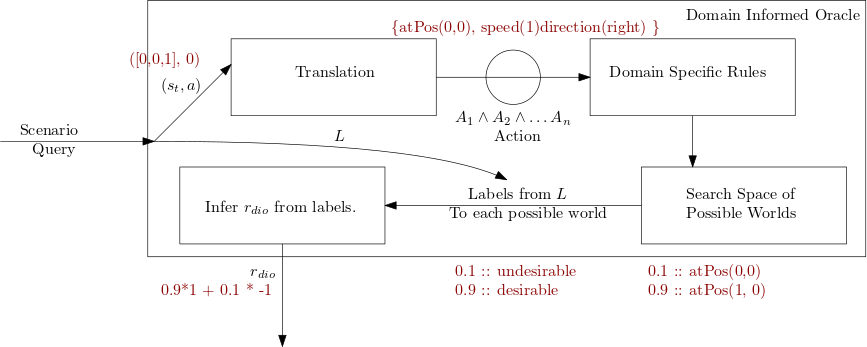
\includegraphics[scale=0.45]{figures/diospecs.png}
  \caption{Step-by-step of Computed Final Reward}
  \label{fig:diospecs}
\end{figure}

It is the case that this reward has to be 'normalized' to the weight of a step. Indeed, suppose there are $S$ possible states for the agent to be at. 
The accumulated reward of the steps should at most equal that of the terminal states. Thus, the final reward, 
\[
  r_{\dio{}} = \dfrac{r'_{\dio{}}}{S} \text{    and    }
  R = r_{rl} + \alpha r_{\dio{}}
\] 
Note that the final reward from \dio{} is added considering some $\alpha$. This is precisely for comparison purposes, i.e. how much value should we given the logic programming module 
to inform a step. 

